% Number squares paper for 18.821 Fall 2012 project 2.
% Authors: Daniel Grazian, Michael Mekonnen, Agustin O Venezuela III

\documentclass[12pt]{amsart}

% Keep everything here in alphabetical order, please! :) -jven

% Packages

\usepackage{amssymb}
\usepackage{graphicx}

% Enumeration

\newtheorem{theorem}{Theorem}[section]

\newtheorem{conjecture}[theorem]{Conjecture}
\newtheorem{corollary}[theorem]{Corollary}
\newtheorem{definition}[theorem]{Definition}
\newtheorem{example}[theorem]{Example}
\newtheorem{examples}[theorem]{Examples}
\newtheorem{lemma}[theorem]{Lemma}
\newtheorem{proposition}[theorem]{Proposition}
\newtheorem{remarks}[theorem]{Remarks}
\newtheorem{remark}[theorem]{Remark}

% Utility commands

% Integers
\newcommand{\z}{\mathbb{Z}}
% Non-negative integers
\newcommand{\znn}{\mathbb{N}}
% Positive integers
\newcommand{\zp}{\mathbb{Z}^+}

\title{Number Squares}
\author{Daniel Grazian, Michael Mekonnen, Agustin O Venezuela III}
\date{October 23, 2012}

\begin{document}

\begin{abstract}
\end{abstract}

\maketitle

\section{Introduction\label{sec:intro}}

In this paper, we present an operation that acts on $4$-tuples of integers in a very simple way. Our aim is to completely understand the behavior of this operation under various starting $4$-tuples.

Our analysis has resulted in a number of observations (and of course corresponding proofs). First, we will show that for any choice of the initial $4$-tuple, continual application of the operation eventually yields the $4$-tuple of all zeroes after finitely many steps. We also provide an upper bound on the number of applications of the operation that are necessary to reach this zero state, given any starting $4$-tuple. Second, we will show that given any non-negative integer $n$, we can construct a starting $4$-tuple such that exactly $n$ applications of the operation yield the zero state. Finally, we look at interesting generalizations of this problem, such as tuples of different lengths and tuples of elements of non-integers.

\section{Definitions and Notation\label{sec:defs}}

We will now define the operation that was introduced in the previous section. Herein, we will use $\znn$ to denote the non-negative integers and $\zp$ to denote the positive integers.

\begin{definition}
Given a $4$-tuple $(a, b, c, d)\in \mathbb{Z}^4$, the \underline{difference} of $(a, b, c, d)$ is the $4$-tuple $(|a - b|, |b - c|, |c - d|, |d - a|)$.
\end{definition}

As motivated in the introduction, we are interested in repeatedly applying the difference to a $4$-tuple until we reach the tuple consisting of all zeroes. In particular, we have the following definition:

\begin{definition}
Given a $4$-tuple $(a, b, c, d)\in \mathbb{Z}^4$, the \underline{(a, b, c, d) game} is the (possibly infinite) sequence of $4$-tuples $\big((a_i, b_i, c_i, d_i)\big)$, generated as follows:

\begin{enumerate}
\item $(a_0, b_0, c_0, d_0) = (a, b, c, d)$
\item $\forall i\in \znn$, if $(a_i, b_i, c_i, d_i) = (0, 0, 0, 0)$, then the $(a, b, c, d)$ game is a finite sequence ending at $(a_i, b_i, c_i, d_i)$. Otherwise, $(a_{i+1}, b_{i+1}, c_{i+1}, d_{i+1})$ is the difference of $(a_i, b_i, c_i, d_i)$.
\end{enumerate}

We will often refer to a $4$-tuple as a game itself, where it is understood that we mean the game whose first element is this $4$-tuple.

\end{definition}

Note that by this definition, the game of a $4$-tuple is either finite ending in $(0, 0, 0, 0)$ or infinite and never containing $(0, 0, 0, 0)$. Naturally, we will refer to the length of a game, meaning the (possibly infinite) length of the sequence.

\section{Finiteness of All Games\label{sec:convergence}}

We will now show that any game $(a,b,c,d)$ starting with four integers $a$, $b$, $c$, and $d$ is finite, i.e. the game terminates at the $4$-tuple $(0,0,0,0)$ in finite time (actually, as we will see, very quickly).

Before proving this claim, let us make two simplifying observation.

First, regardless of the elements in the first $4$-tuple of a game, by definition of the difference operation, the second $4$-tuple in the game will have non-negative elements. Thus, for simplicity, henceforth we will assume that all the elements in the starting $4$-tuple of a game are non-negative, for if they are not, we can just consider the game starting from the difference of the $4$-tuple.

Second, note that the games $(a,b,c,d)$ and $(b,c,d,a)$ have exactly the same length. That is, rotating a $4$-tuple does not alter the properties of the game other than changing the order of numbers as they appear in the $4$-tuples in the game. The reason for this is the cyclic nature of the difference operation: the difference of $(b,c,d,a)$ contains the same elements that are in the difference of $(a,b,c,d)$, but rotated left by $1$. Thus, the lengths of the two games are equal.

Equipped with these simplifications, we can now embark upon a proof of our claim. Let us first prove a much simpler, yet very useful, statement of the claim.

\begin{lemma}
All games starting with $4$-tuples only containing $0$'s and $1$'s have length at most $5$.
\label{lem:zerosones}
\end{lemma}

\begin{proof}
Indeed there are $16$ $4$-tuples that contain only $0$'s and $1$'s. However, we only need to consider $6$ of them, namely $(0,0,0,0)$, $(0,1,1,1)$, $(1,0,0,0)$, $(1,0,0,1)$, $(1,0,1,0)$, and $(1,1,1,1)$, since the other $10$ $4$-tuples can be obtained by appropriate rotation of one of these $6$. Based on our observation above that a rotation does not affect the length of a game, studying these $6$ $4$-tuples is sufficient.

\begin{figure}
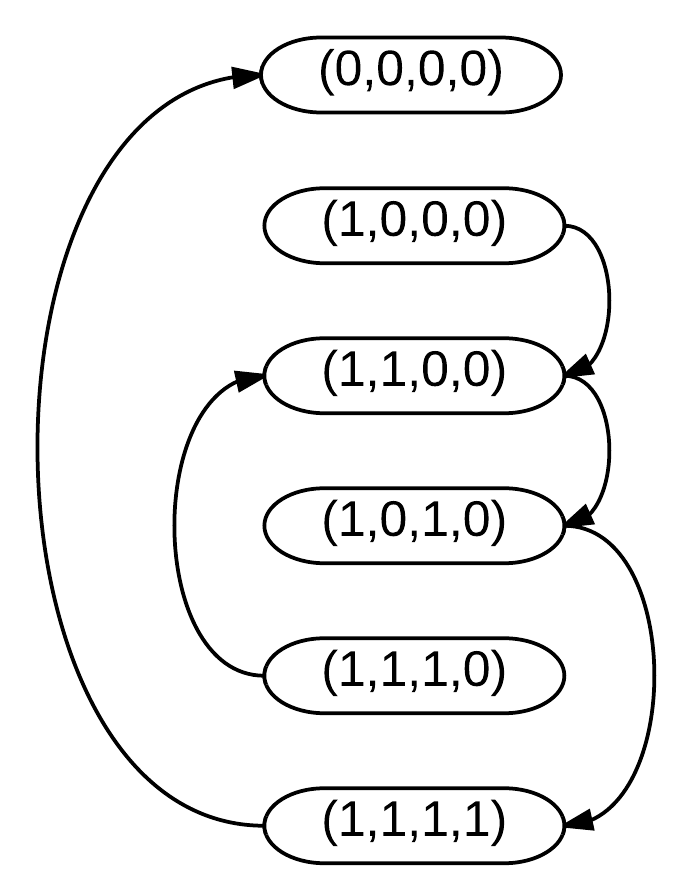
\includegraphics{number_squares_0s_and_1s.png}
\caption{All games starting with just $0$'s and $1$'s have length at most $5$.}
\label{fig:zerosones}
\end{figure}

Figure \ref{fig:zerosones} shows a graph in which the nodes represent the $6$ $4$-tuples we are studying, and an edge from node $A$ to node $B$ indicates that the difference of $A$ is $B$. From this graph, it is clear that all of the games have finite length. Furthermore, the maximum length of such a game is $5$ (length $5$ is achieved by $(0,1,1,1)$ and $(1,0,0,0)$).

\end{proof}

We can use Lemma \ref{lem:zerosones} to make a stronger claim.

\begin{lemma}
For any $n \in \znn$, if four integer $a$, $b$, $c$, and $d$ are congruent to $0$ modulo $2^n$, then the $4$-tuple $(a_4, b_4, c_4, d_4)$ in the $(a,b,c,d)$ game will have elements that are congruent to $0$ modulo $2^{n+1}$.
\label{lem:evenodd}
\end{lemma}

\begin{proof}
Since $a$, $b$, $c$, and $d$ are congruent to $0$ modulo $2^n$, each is congruent to either $0$ or $2^n$ modulo $2^{n+1}$. Now define $\hat{a}$ to be $0$ if $a$ is congruent to $0$ modulo $2^{n+1}$ or $1$ otherwise. That is,
$$
\hat{a} = \frac{a \bmod{2^{n+1}}}{2^n}
$$
Similarly define $\hat{b}$, $\hat{c}$, and $\hat{d}$. Now if we look at the game $(\hat{a},\hat{b},\hat{c},\hat{d})$, it precisely captures whether the corresponding elements in the corresponding 4-tuples in the game $(a,b,c,d)$ are congruent to $0$ or $2^n$ modulo $2^{n+1}$. By Lemma \ref{lem:zerosones}, we know that the game $(\hat{a},\hat{b},\hat{c},\hat{d})$ terminates at $(0,0,0,0)$ after at most $5$ steps, so we know that the elements in the game $(a,b,c,d)$ will be congruent to $0$ modulo $2^{n+1}$ after at most $5$ steps.
\end{proof}

We can use this to make two conclusions that will prove our main result and also give an upper bound on the length of any game.

\begin{corollary}
For any $n \in \znn$, the $4$-tuple $(a_{4n}, b_{4n}, c_{4n}, d_{4n})$ in the $(a,b,c,d)$ game has elements that are congruent to $0$ modulo $2^n$.
\label{cor:pow2}
\end{corollary}

\begin{proof}
We prove this by induction on $n$.
Both the base case and inductive step of this inductive proof follow directly from Lemma \ref{lem:evenodd}.
\end{proof}

\begin{corollary}
Let $M=\max(a,b,c,d)$. Then the game $(a,b,c,d)$ has length at most $4\lceil\log_2{M}\rceil + 1$.
\end{corollary}

\begin{proof}
Let $n = \lceil\log_2{M}\rceil$. By Corollary \ref {cor:pow2}, the $4$-tuple $(a_{4n}, b_{4n}, c_{4n}, d_{4n})$ in the $(a,b,c,d)$ game has elements that are congruent to $0$ modulo $2^n$. However, since $M\leq2^n$, this implies that $a_{4n}=b_{4n}=c_{4n}=d_{4n}=0$.
\end{proof}

\section{Existence of Arbitrarily Long Games\label{sec:longgames}}

The previous section argued that all games are of finite length. However, we will show in this section that games may be of any arbitrarily long finite length. We state this more precisely in the following theorem:

\begin{theorem}
For all $n\in \zp$, there exists a game of length $n$.
\end{theorem}

For $n < 5$, it is very easy to construct such a game. Indeed, for $n=1,2,3,4$ we have the games $(0, 0, 0, 0)$, $(1, 1, 1, 1)$, $(1, 0, 1, 0)$, and $(1, 1, 0, 0)$, respectively.

Our plan for $n \geq 5$ is as follows: given games of a particularly nice form, we will show how to construct a game of one greater length while still preserving this form. The result is that this construction can be repeated indefinitely until a game of the desired length is reached. First, we need the following lemma:

\begin{lemma}
Suppose the game $(a, b, c, d)$ has length $n$. Then the games $(ua, ub, uc, ud)$ and $(a + v, b + v, c + v, d + v)$ for any $u, v\in \mathbb{Z}$, $u\neq 0$, also have length $n$.
\end{lemma}

\textit{Proof:} Suppose the $(a, b, c, d)$ game is $\Big((a_i, b_i, c_i, d_i)\Big)_{i=0}^{n - 1}$. Then it is clear that for $u\neq 0$, the $(ua, ub, uc, ud)$ game is $\Big((|u|a_i, |u|b_i, |u|c_i, |u|d_i)\Big)_{i=0}^{n - 1}$. Similarly, the difference of $(a + v, b + v, c + v, d + v)$ is the same as that of $(a, b, c, d)$. The result follows.

Returning to the original proof, consider a game $(0, a, b, c)$ of length $n$, where $0\leq a\leq b\leq c$ and $a + b < c$. Alter this game by doubling each element, then adding $c - b - a$ to each element. This yields the game:

$$\begin{array}{cl}
& (c - b - a, 2a + (c - b - a), 2b + (c - b - a), 2c + (c - b - a)) \\
= & (-a - b + c, a - b + c, -a + b + c, -a - b + 3c)
\end{array}$$

By the lemma above, this game also has length $n$. Furthermore, since each element of this tuple is non-negative (and in fact positive), it is the difference of the following sequence:

$$(0, -a - b + c, -2b + 2c, -a - b + 3c)$$

This game thus has length $n + 1$ since its difference yields a game of length $n$. Note also that this tuple is again of the form $(0, a', b', c')$, where $0\leq a'\leq b'\leq c'$ and $a' + b' = -a - 3b + 3c < -a - b + 3c = c'$. Thus we may iterate this process to yield a game of length $n + 2$, and so on.

It thus remains to provide a game of the desired form of length $5$. The game $(0, 1, 1, 3)$ works, and we're done. $\qed$

Note that our proof is constructive: given any $n\in \zp$, the proof gives an algorithm (and an efficient one at that) to find a length $n$ game. As an example, starting with the length $5$ game $(0, 1, 1, 3)$, we find that a length $50$ game is:

$$(0, 103502633381134336, 293873656088494080, 644020556730990592)$$

TODO(jven): Should I motivate this proof a little bit? Could be a little long-winded.

\section{Games For Other $k$-tuples}

This paper is primarily concerned with games of 4-tuples, but it is worth exploring the behavior of games of other sizes. We will show that given a an integer $n$, every game of size $n$ terminates if and only if $n$ is an integer power of 2.

First, we prove a useful Lemma:

\begin {lemma}
Consider the game $(a_0, a_1, a_2, \ldots, a_n)$ where n is even (so the number of elements is odd) and the elements are not all equal. Let the game include a non-zero even number of odd elements. Then the game never terminates.
\label{lem:evenodds}
\end{lemma}

\begin{proof}
\emph{Notice that the difference of any tuple must include an even number of odd elements} (1). The number of odd elements is precisely the number of pairs of adjacent elements (with the initial and final elements considered adjacent) consisting of an even and an odd element. Walking along the tuple from $a_0$ to $a_n$ and back around to $a_0$, every even element immediately followed by an odd element must be matched by an odd element immediately followed by an even element, and vice versa. So there is an even number of such pairs and thus an even number of odd elements in the difference of the tuple.

Let $G_0$ be the initial game state described in the statement of the lemma and let $G_{i+1}, i \geq 0$ be the difference of $G_i$. We show by induction on $i$ that the game never terminates:

$G_0$ includes an even number of odd elements, by construction. Assume that $G_i$ includes a non-zero even number of odd elements. So $G_i$ includes both even and odd elements and therefore must have adjacent even and odd elements. Therefore, $G_{i+1}$ must include a non-zero number of odd elements, and that number must be even, by (1). So $G_{i+1}$ cannot be the tuple of all $0$'s. This concludes the proof of the lemma.
\end{proof}

Lemma \ref{lem:evenodds} shows that for every odd $n > 1$ there are games of size $n$ that do not terminate. For example, (1,1, 0 \ldots, 0), with an odd number of 0's, does not terminate. We now use this result to show that for every $n$ that is not an integer power of 2, there are games of size $n$ that do not terminate.

We need one more lemma to prove our claim:

\begin{lemma}
\label{lem:doubles}
If $(a_0, a_1, \ldots, a_{n})$ is a game that does not terminate, then $(a_0, a_1, \ldots, a_n, a_0, a_1, \ldots, a_n)$ also does not terminate.
\end{lemma}

\begin{proof}

The difference of $(a_0, a_1, \ldots, a_{n})$ is:

\noindent
 $(|a_0 - a_1|, |a_1 - a_2|, \ldots, |a_{n-1} - a_n|, |a_n - a_0|)$.

\vspace{.2cm}

The difference of $(a_0, a_1, \ldots, a_{n}, a_0, a_1, \ldots, a_n)$ is:

\noindent
$(|a_0 - a_1|, |a_1 - a_2|, \ldots, |a_{n-1} - a_n|, |a_n - a_0|$,

\noindent
$|a_0 - a_1|, |a_1 - a_2|, \ldots, |a_{n-1} - a_n|, |a_n - a_0|)$.

Since this is true for general values of $a_0$, \ldots, $a_n$, the $i$th sequence in the game beginning with $(a_0, a_1, \ldots, a_{n}, a_0, a_1, \ldots, a_n)$ is simply

\noindent
two appended copies of the $i$th sequence in the game beginning with $(a_0, a_1, \ldots, a_{n})$. So if $(a_0, a_1, \ldots, a_{n})$ doesn't terminate, then 

\noindent
$(a_0, a_1, \ldots, a_{n}, a_0, a_1, \ldots, a_{n})$ doesn't terminate.

\end{proof}

\begin{theorem}
\label{theorem:notPowersOfTwo}
If $n$ is an integer that is not an integer power of 2, then there is a game of size $n$ that does not terminate.
\end{theorem}

\begin{proof}

Given an integer $k > 2$ that is not an integer power of 2, $k$ can be written in the form $p \times 2^{m}$ where $p$ is an odd prime and $m$ is an integer. By Lemma \ref{lem:evenodds}, there is a game of size $p$ that does not terminate (e.g. $(1,1,0, \ldots, 0)$) By applying Lemma \ref{lem:doubles} $m$ times, we obtain a game of size $m$ that does not terminate. 
\end{proof}

TODO (Daniel) Prove that games of size $k = 2^n$ always terminate.



\section{Games Over Non-Integers}

We will return from our investigation of $k$-tuples in the previous section and again focus on $4$-tuples. To begin, we will extend our notion of a game to allow for $4$-tuples of rational numbers.

\begin{theorem}
All games of $4$-tuples over $\mathbb{Q}$ are finite.
\end{theorem}

The proof of this follows very easily from the fact that game length is invariant under the operation of scaling each element of the $4$-tuple by a non-zero quantity. We used this fact in our construction of arbitrarily long games in Section $\ref{sec:longgames}$. (Note that the lemma in that section dealt only with integers but the argument is easily extended to any reals.)

Indeed, given a game $\left(\dfrac{a}{p}, \dfrac{b}{q}, \dfrac{c}{r}, \dfrac{d}{s}\right)$ over rationals, it is clear that the game will progress the same as the game $(a, b, c, d)$ over the integers, with each tuple in the sequence scaled by $\dfrac{1}{pqrs}$. The result follows.

A more interesting question arises when we instead consider game of $4$-tuples over $\mathbb{R}$.

\section{Games Over the Real Numbers}

Our results regarding games over the real numbers are not as thorough as our results on games over the integers, but we did make some interesting discoveries. Note that in this section, \emph{all games are games of 4-tuples}.

We discovered a large class of terminating games over the reals. We also discovered examples of games over the reals which do not terminate. This contrasts with games over the integers, which always terminate.



TODO(jven,dgrazian): Solve me! :D

\section{Non-terminating $4$-tuple Games\label{sec:nonterminating}}

TODO(mikemeko) naming this section might not be necessary.

We have shown that $4$-tuple games that start with $4$ rational numbers always terminate. Now we will demonstrate, by example, that there exist $4$-tuple games that actually do not terminate.

Consider the game
$$
(1,x,x^2,x^3)
$$
where $x$ is a real number greater than $1$ that we will define shortly. Note that the difference of this $4$-tuple is
\begin{align*}
& (x-1, x^2 - x, x^3 - x^2, x^3 - 1)\\
= & (x-1) (1, x, x^2, x^2 + x + 1).
\end{align*}
If we choose $x$ such that $x^2 + x + 1 = x^3$, then we see that the difference of $(1,x,x^2,x^3)$ is a multiple of itself, which shows us that the game will never terminate. The only real (and irrational) solution to $x^2 + x + 1 = x^3$, which is approximately $1.839$, satisfies the condition of being greater than $1$, so we have indeed constructed a non-terminating $4$-tuple game.
\end{document}